
\chapter{Introducción al scraping en la web: Marco teórico}
\label{cha:introduccion al scraping en la web}

Comienzo del trabajo...aaaa

\section{¿Que es el web scraping?}
\label{sec:Que es el web scraping}


Para acceder a la API de Twitter, como se indica en la documentación de la misma, existen dos métodos de 
acceso Oauth2 y Oauth1a. El acceso con cada uno de ellos dependerá del tipo de información que se desee 
extraer \cite{oauth1a}. Como veremos a continuación, el método de acceso elegido será Oauth1a.

\begin{figure}[tphb]
  		   \centering
     		   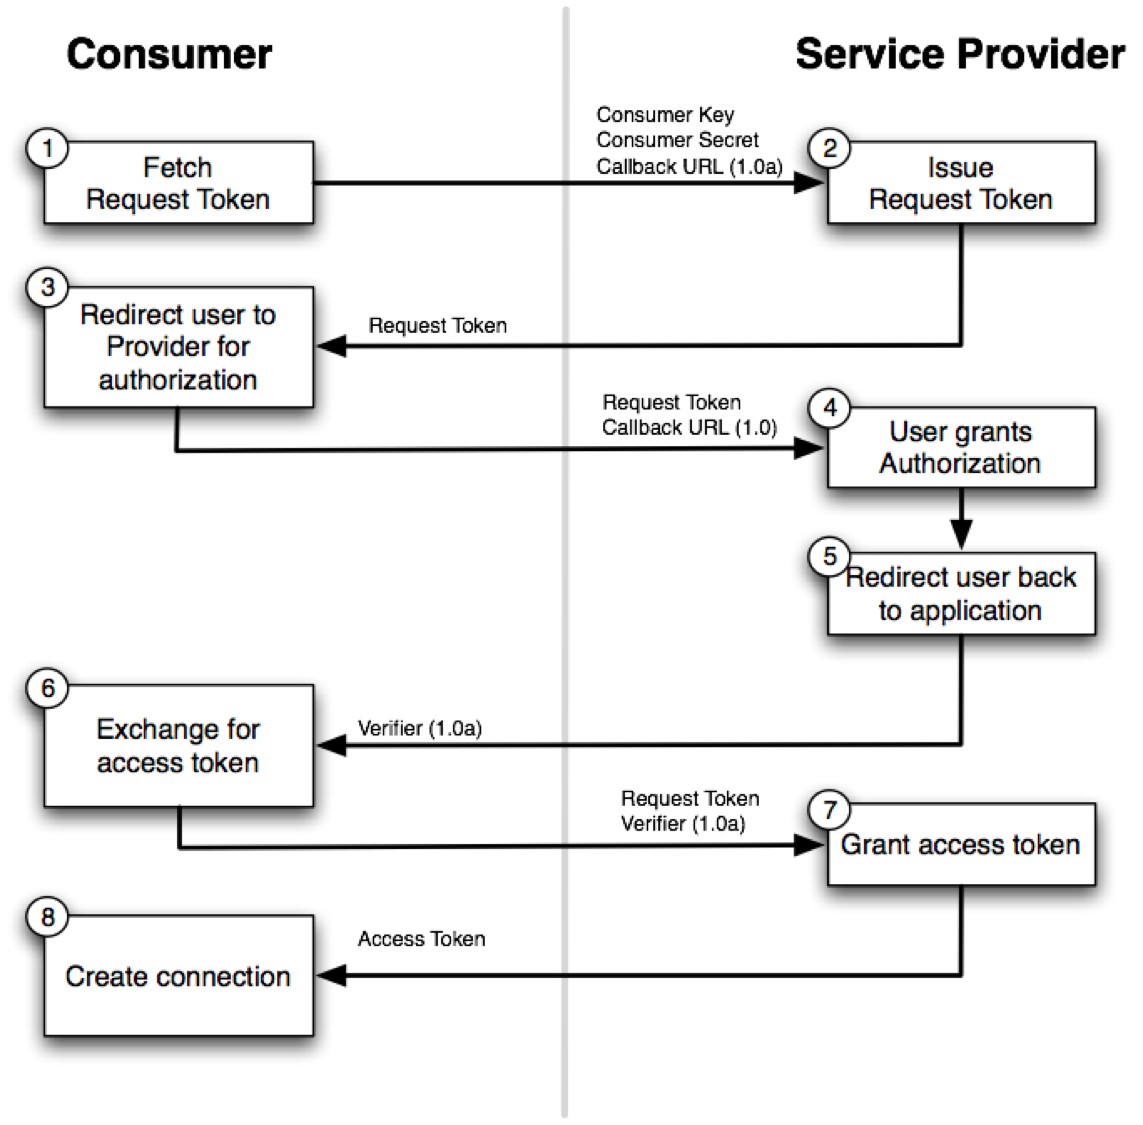
\includegraphics[width=4.5in]{Oauth1a.png}
  		   \caption{Funcionamiento de Oauth1a}
  		   \label{img:oauth1a}
\end{figure}






